


\chapter{GPU通用计算简介}

\TODO GPU通用计算发展历史简述。

现在较为成熟和广泛使用的GPU编程技术是NVIDIA公司在2007年提出
的CUDA(Compute Unified Device Architecture)编程模型,
以下主要对CUDA进行介绍。

\section{CUDA简介}

\subsection{CUDA总体设计}

CUDA翻译为\emph{统一计算设备架构},本身定位做一种包含CPU和GPU的编程模型,
不过实际上一般只用作GPU编程和GPU、CPU通讯编程。

为方便起见本章以下只考虑单机上只有一个GPU核心的情况,
多GPU核心情况的讨论放在\sectionref{sec:gpu.multi-gpu}进行。

CUDA把设备资源分为主机端和GPU端两部分,
主机端包含CPU、内存等正常C/C++程序可以访问到的资源,
GPU端包含多个SM(Streaming Multiprocessor)
或SMX(Next Generation Streaming Multiprocessor)
\footnote{从 NVIDIA显卡的 Kepler 架构开始,SM的规格大幅改变,改称为SMX。}
、显存等资源。

其中SM/SMX代表GPU核心内的一个相对独立的向量处理单元,
类似传统的向量机中央处理器,这些SM/SMX位于GPU的核心芯片内。
显存位于显卡PCB上,并被所有的SM/SMX共享。

显存和主机内存是独立的,有各自的地址空间,
CPU端的代码不能直接读写显存,
GPU端的代码也不能直接读写内存,
需要程序员手工在显存和内存之间做数据传输。
CUDA允许在主机端申请所谓的\emph{页锁定主机内存}(Page-Locked Host Memory),
并允许GPU端直接访问,
由显卡驱动负责在内存和显卡之间进行自动数据传输。
此外,对于通用计算专用的Tesla显卡,
CUDA可以开启Unified Virtual Address Space功能,
即对内存和显存统一编址访问,可以省去一些编程上的繁琐操作。
\cite{cudadoc-cprogrammingguide}

\subsubsection{Global函数}

GPU上执行的代码需要放在专门的Kernel函数中,
这些函数在CUDA使用\_\_global\_\_进行标识,所以又称global函数。
Global函数只能由CPU端的代码通过特殊方式调用。
在CUDA 5.0之前global函数间不能相互调用,
global函数只能调用一种有\_\_device\_\_标识的函数(以下称为device函数)。
CUDA 5.0引入了Dynamic Parallelism功能,
允许在global函数内调用global函数,并定义了对应的语义,
该功能依赖计算能力\footnote{NVIDIA对其发布的GPU核心的功能进行划分的标准,当前Kepler架构的计算能力为3.0-3.5。}%
为3.5的GPU核心(如GK110,对应的显卡有GTX Titian、Tesla K20等),
详见文献\onlinecite{cudadoc-dynamicparallelism}。

Global函数是GPU上运行的程序的最基本单元,虽然global函数可以调用device函数,
但被调用的device函数的各种运行时配置都是依赖于直接或间接调用它的global函数。

Global函数实际运行时可以被一组线程同步执行,类似传统的向量机,
同步执行的线程数量在调用global函数的时候进行设置。

CUDA将运行一个global函数的线程分Grid、Block两个层级进行组织:
Grid代表所有参与的线程,一个Grid包含一个或多个Block,每个Block在Grid内都有自己的编号,
CUDA提供的Block编号可以是1维、2维或3维整数;
一个Block又包含一个或多个Thread,每个Thread在Block内也有自己的编号,
CUDA提供的Thread编号同样是1维、2维或3维整数,
这里的Thread就是一个实际的硬件线程,有自己的寄存器组等资源。
一个实际的线程组设置见\floatref{fig:gpu.cuda.blocks}。

\begin{figure}
\centering
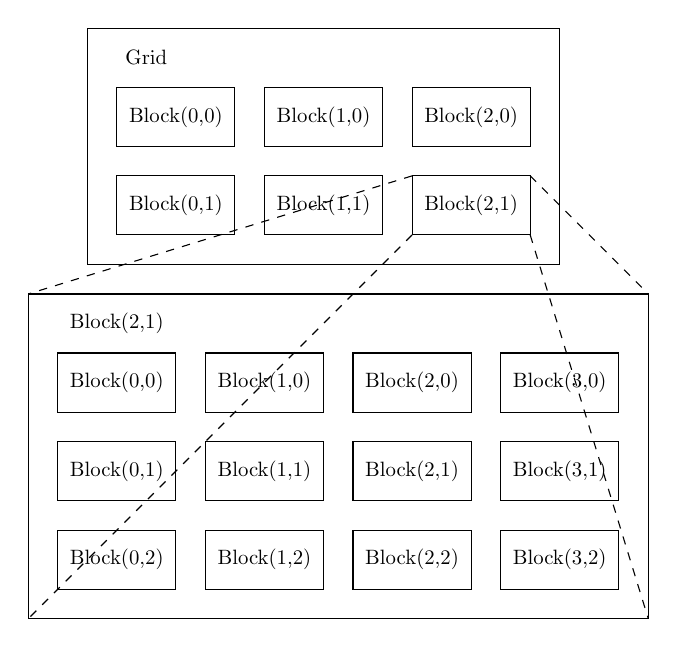
\begin{tikzpicture}[scale=0.75, transform shape]
\def\TextBox#1#2#3{
\draw  (#1,#2) rectangle (#1+2,#2+1);
\node at (#1+1, #2+0.5) {#3};
}

\foreach \x in {0,...,2}
  \foreach \y in {0,...,1}
  {
    \TextBox{\x*2.5+1}{-\y*1.5+3}{Block(\x,\y)}
  }
\draw  (0.5,5) rectangle (8.5,1);
\node at (1.5,4.5) {Grid};

\foreach \x in {0,...,3}
  \foreach \y in {0,...,2}
  {
    \TextBox{\x*2.5}{-\y*1.5-1.5}{Block(\x,\y)}
  }
\draw  (-0.5,0.5)  rectangle (10,-5);
\node at (1,0) {Block(2,1)};

\draw [dashed]  (6,2.5) edge (-0.5,0.5);
\draw [dashed]  (8,2.5) edge (10,0.5);
\draw [dashed]  (6,1.5) edge (-0.5,-5);
\draw [dashed]  (8,1.5) edge (10,-5);
\end{tikzpicture}
\caption[线程组层次结构示意图]{\label{fig:gpu.cuda.blocks}线程组层次结构示意图
\cite{cudadoc-cprogrammingguide}}
\end{figure}

同一个global函数调用时所涉及的线程均使用global函数的参数作为输入,
CUDA提供threadIdx、blockIdx等变量在代码中区分各个线程。
线程以Block为单元分配给GPU上的各个SM/SMX独立执行,
Block之间没有任何直接的同步方式,
程序员不需要知道也不应该猜测各Block是如何在各个SM/SMX执行的。
需要说明的是:强行使用显存作为Block间的同步可能会导致各SM/SMX死锁。
实际Block间同步的最主要方式就是等待该global函数执行完,
此时所有Block状态都是确定的,即已经执行完。

这样GPU或驱动就可以根据实际GPU核心上的SM/SMX数量来具体配置各Block是如何在SM/SMX上执行的,
使得当SM数量不超过Block数量时global函数有了一定的并行扩展性,
见\floatref{fig:gpu.cuda.scalability}。
由于每个Block是运行在一个实际SM/SMX上的,
所以SM/SMX的寄存器、共享存储空间等资源会对Block的大小(包含的Thread数量)有一定的限制,
而CUDA对Grid大小(包含的Block数量)的限制则很小。
NVIDIA这样做是为了通过强制程序员对计算任务进行分割的方式获得了一定的程序并行扩展性,
同时也简化了同一系列不同规格GPU的设计,即通过增减SM/SMX的数量来控制GPU计算能力。
\begin{figure}
\centering
\begin{tikzpicture}[scale=0.6, transform shape]
\def\TextBox#1#2#3{
\draw  (#1,#2) rectangle (#1+2,#2+1);
\node at (#1+1, #2+0.5) {#3};
}

\foreach \x in {0,...,3}
  \foreach \y in {0,...,1}
  {
    \TextBox{\x*2.5+1}{-\y*1.5+3}{Block(\x,\y)}
  }
\draw  (0.5,5) rectangle (11,1);
\node at (3,4.5) {\large Kernel函数的Grid};

\draw [dashed] (-3,-4) -- (16.5,-4);

\draw  (-1,-3.5) rectangle (4.5,-1);
\node at (1.5,-1.5) {\large 2个SMX的GPU};
\draw [-latex new, arrow head=3mm] (7,1) -- (9.5,-1);
\foreach \x in {0,...,1}
{
  \TextBox{\x*2.5-0.5}{-3}{SMX \x}
}
\foreach \t in {0,...,3}
{
  \foreach \x in {0,...,1}
  {
    \TextBox{\x*2.5-0.5}{-\t*2-6}{Block(\t,\x)}
  }
  \draw  (-1,-\t*2-4.75) rectangle (4.5,-\t*2-6.25);
}

\draw  (5.5,-3.5) rectangle (16,-1);
\node at (8,-1.5) {\large 4个SMX的GPU};
\draw [-latex new, arrow head=3mm] (3.5,1) -- (2,-1);
\foreach \x in {0,...,3}
{
  \TextBox{\x*2.5+6}{-3}{SMX \x}
}
\foreach \t in {0,...,1}
{
  \foreach \x in {0,...,3}
  {
    \TextBox{\x*2.5+6}{-\t*2-6}{Block(\x,\t)}
  }
  \draw  (5.5,-\t*2-4.75) rectangle (16,-\t*2-6.25);
}

\draw [dashed,-latex new, arrow head=3mm] (-1.5,-4.5) -- (-1.5,-13);
\foreach \t in {0,...,3}
{
  \node at  (-2.5,-\t*2-5.5) {\Large t=\t};
}

\draw (5,-0.5) -- (5,-12.5);
\end{tikzpicture}
\caption[CUDA程序的扩展性示意图]{\label{fig:gpu.cuda.scalability}CUDA程序的扩展性示意图
\cite{cudadoc-cprogrammingguide}}
\end{figure}

总的来说,GPU核心相当于一组不能单独编程的、以显存作为共享存储器的、带有自动负载平衡的小型向量机组。


\subsection{CUDA的GPU设备模型}

\begin{figure}
\centering
\begin{tikzpicture}[scale=0.75, transform shape]
%15*SMX
\def\SMX#1#2{
\draw  (#1+0, #2) rectangle (#1+1, #2+1);
\node at (#1+0.5, #2+0.5) {SMX};
}
\def\len{1.5}
\foreach \x in {0,...,8}
{ \SMX{\x*\len}{0} }
\foreach \x in {0,...,7}
{ \SMX{\x*\len+0.75}{-3} }

%L2 Cache
\draw  (0,-0.5) rectangle (13,-1.5);
\node at (6.5,-1) {L2 Cache};


\def\Memory#1#2{
\draw  (#1,#2) rectangle (#1+2,#2+1);
\node at (#1+1,#2+0.5) {\small 显存控制器};
}
\foreach \i in {0,1,2}
{ \Memory{-2.5}{-\i*1.5} }
\foreach \i in {0,1,2}
{ \Memory{13.5}{-\i*1.5} }

\draw  (-2.5,2) rectangle (15.5,1.5);
\node at (6.5,1.75) {线程调度器(GigaThread Engine)};

\draw  (-2.5,3) rectangle (15.5,2.5);
\node at (6.5,2.75) {PCI Express 3.0接口};

\draw  (-3,4) rectangle (16,-3.5);
\node at (-1.5,3.5) {\Large GK110};
\end{tikzpicture}
\caption[GK110结构示意图]{\label{fig:gpu.cuda.gk110}GK110结构示意图
\cite{cudadoc-KeplerGK110ArchitectureWhitepaper}}
\end{figure}

GPU是由多个SMX组成的,例如Kepler架构GK110核心
(结构见\floatref{fig:gpu.cuda.gk110})就包含15个SMX,
其中每个SMX含有192个CUDA Core单元(支持单精度、整数计算)、
64个双精度浮点计算单元、32个特殊函数计算单元、32个读取/存储单元,
4个Wrap调度器,65536个32bit寄存器,见\floatref{fig:gpu.cuda.smx}。
\cite{cudadoc-KeplerGK110ArchitectureWhitepaper}

\begin{figure}
\centering
\includegraphics[scale=0.6]{smx.png}
\caption[SMX结构示意图]{\label{fig:gpu.cuda.smx}SMX结构示意图
\cite{cudadoc-KeplerGK110ArchitectureWhitepaper}}
\end{figure}

The SMX schedules threads in groups of 32 parallel threads called warps.
 Each SMX features four warp schedulers and eight instruction dispatch units,
  allowing four warps to be issued and executed concurrently.
  Kepler’s quad warp scheduler selects four warps,
   and two independent instructions per warp can be dispatched each cycle. 
\cite{cudadoc-KeplerGK110ArchitectureWhitepaper}


\subsection{多GPU及多节点并行计算}
\label{sec:gpu.multi-gpu}

\section{其他GPU编程技术简介}

\subsection{OpenCL}
\subsection{AMP}
\subsection{OpenACC与OpenMP}
